\chapter{Contexto Teórico}
No son los aspectos técnicos para la creación de sistemas de información los que distinguen al SITEM sino las nuevas estructuras de información -y su correlación, las que brindan una novedad en el contexto de la proyección de soluciones en Telemedicina. El presente capítulo provee la base teórica que sustenta dichas estructuras y relaciones, abordando el marco legislativo y demás temáticas que son necesarias para caracterizar los componentes primordiales de los Sistemas de Telemedicina. 

Teniendo en cuenta el caracter evolutivo del proyecto software y como referencia para posteriores desarrollos soportados en el SITEM, también se tratan cuestiones relevantes al proceso de ingeniería que guió el análisis, diseño y elaboración del sistema.

\section{Telemedicina}

La Telemedicina \cite{aim}, \cite{bashshur77}, \cite{itu} se ha convertido rápidamente en un concepto que extiende sus raices etimológicas. El Ministerio de Protección Social colombiano con la \textit{Resolución 1448 del 8 de mayo de 2006} define a la Telemedicina como:
\begin{quote}
“la provisión de servicios de salud a distancia, en los componentes de promoción, prevención, diagnóstico, tratamiento o rehabilitación, por profesionales de la salud que utilizan tecnologías de la información y la comunicación, que les permiten intercambiar datos con el propósito de facilitar el acceso de la población a servicios que presentan limitaciones de oferta, de acceso a los servicios o de ambos en su área geográfica.”
\end{quote} 

Es por tanto un campo multidisciplinar que integra componentes de diferentes áreas del saber que incluye entre otros a la medicina, la ingeniería electrónica, la telemática, la informática, la ingeniería de sistemas, la inteligencia artificial, la biónica, la sicología, la sociología y la antropología. Las redes actuales de Telemedicina consideran elementos que van mucho más alla del simple despliegue de redes tecnológicas de intercomunicación y evidentemente se plantean como redes de interacción social cuyo objetivo primario - más no el único, es la prestación de servicios médicos apoyadas en las TIC.

Dependiendo el grado en que se presente cada uno de los elementos mostrados en la figura ~\ref{elementosred} y de la mayor o menor correlación entre ellos, se pueden crear sistemas de Telemedicina que se acerquen al ideal de proveer servicios de salud de alta calidad. Dichos sistemas, aunque dinámicos y evolutivos, deberán mantener una estructura nuclear cuyas propiedades generales son según \cite{bashshur95}: 
\begin{enumerate}
\item Separación geográfica entre el proveedor y el cliente durante un encuentro clínico o entre dos o más proveedores.
\item Utilización de tecnologías informáticas y de comunicaciones para realizar la interacción. 
\item Equipo humano/técnico de gestión del sistema. 
\item Desarrollo de una infraestructura organizacional. 
\item Desarrollo de protocolos clínicos para orientar a los pacientes hacia diagnósticos y fuentes de tratamiento apropiados. 
\item Normas de comportamiento que reemplazan las normas del comportamiento presenciales.
\end{enumerate}

\begin{figure}
 \centering
 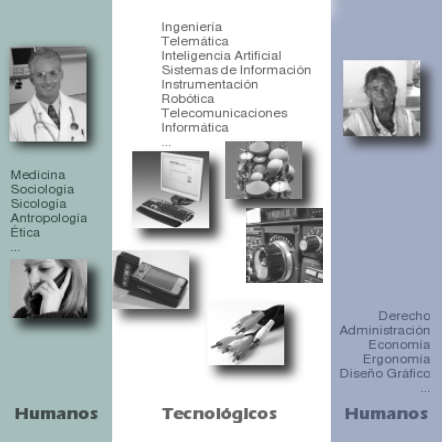
\includegraphics[width=156mm, height=156mm]{sistema_telemedicina.png}
 \caption{Elementos genéricos y áreas del saber de una red de Telemedicina}
 \label{elementosred}
\end{figure}

La Telemedicina es catalogada siguiendo básicamente criterios de \cite{oas2002}: sincronización temporal entre el proveedor y el cliente -diferida o en tiempo real; servicios de salud que se presten \cite{aparicio2000} - consulta, diagnóstico, atención, seguimiento, educación, administración, etc;  o especialidad médica que se trate - radiología, patología, cardiología, dermatología, etc. La catalogación siempre es independiente de la red tecnológica y de comunicaciones sobre la cual se despliegue.

\subsection{Componentes Tecnológicos de los Sistemas de Telemedicina}
La fase actual del SITEM se centra en dos conjuntos básicos de componentes de los sistemas de Telemedicina, los médicos y los tecnológicos. Debido al perfil de profesionales que han participado en el desarrollo, los elementos tecnológicos han sido mejor caracterizados hasta el momento.

\begin{figure}
 \centering
 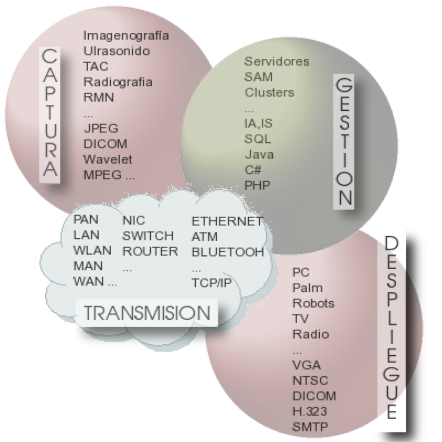
\includegraphics[width=156mm, height=156mm]{red_1.png}
 \caption{Subsistemas Tecnológicos Básicos en un Sistema de Telemedicina}
 \label{subsistemas}
\end{figure}


Para efectos de facilitar su análisis y modelado, en la dimensión puramente tecnológica, un sistema de Telemedicina puede reducirse a cuatro subsistemas \cite{aparicio2003}:

\begin{itemize}
 \item \textbf{Captura de datos:} Conformado por los dispositivos de hardware, los protocolos y aplicaciones software que trabajan conjuntamente para transformar información médica en datos susceptibles de ser administrados usando técnicas digitales.
 \item \textbf{Transmisión de Datos:} Hacen parte de este subsistema los dispositivos de hardware, las tecnologías de interconexión, los protocolos y aplicaciones que permiten estructurar redes de transmisión de datos digitales de una manera fiable en tiempos aceptables para un servicio específico.
 \item \textbf{Gestión de Información:} Dispositivos de hardware - computadores, sistemas de almacenamiento masivo, etc; y  sistemas de información que almacenan, procesan, distribuyen y analizan la información proveniente de los subsistemas de captura de datos.
 \item \textbf{Despliegue de información:} Elementos de hardware (pantallas, transductores, sistemas de audio, etc), aplicaciones software y protocolos asociados que permiten recibir y reproducir la información médica. 
\end{itemize}

Todos ellos necesariamente interrelacionados por medio de interfaces y protocolos definidos; El uso de estándares abiertos es de vital importancia para permitir que los sistemas de Telemedicina puedan ser interoperables, esto se ha logrado en gran medida en el subsistema de transmisión de datos pero aún se encuentran serios problemas en los demás subsistemas debido al sinnúmero de patentes y protocolos propietarios que las empresas fabricantes de dispositivos médicos aún ostentan.
\section{Marco Legislativo y Normativo}

OpenSITEM es un sistema que gestiona información sobre diferentes áreas del saber de acuerdo a las categorías de los nodos que se definan. Cada aspecto (atributos, interfaces, interoperaciones) está en un marco legislativo y normativo concreto, o está asociado a estándares y normas de uso extendido o de facto aceptadas en el mundo. La información de OpenSITEM que sea de acceso público no podrá incluir protección por derechos de autor que restrinjan su difusión \cite{congreso565},\cite{congreso23}. Debido a esto, el código fuente de OpenSITEM es cubierto por una licencia abierta que se ciñe a la normatividad expresada en la Ley 565 de 2000: adopción del Tratado de la OMPI sobre Derechos de Autor y complementarias para garantizar que todos los aspectos tanto técnicos como conceptuales estén debidamente registrados \cite{congreso565},\cite{congreso44},\cite{congreso1360}. 

OpenSITEM es una plataforma para la definición de nodos y no es posible \textit{a priori} definir el marco legislativo que regirá cada nodo o categoría. Sin embargo, se describe a continuación un marco relacionado con las categorías base que se han definido en el primer modelo del sistema.

\subsection{En el Ámbito de los Servicios Médicos}

El Derecho a la Salud ha sido reconocido por normas y pactos internacionales contenidos en tratados sobre Derechos Humanos, Económicos, Sociales, y Culturales  (DHESC). Esos acuerdos han sido ratificados por Colombia para su cumplimiento como un derecho de los ciudadanos. “La Corte Constitucional; ha señalado que el inciso segundo del artículo 93 de la Carta Política confiere rango constitucional a todos los tratados de derechos humanos, económicos,  sociales y culturales, ratificados por Colombia y referidos a derechos que ya aparecen en la Carta” \cite{sentencia1319} como ocurre con el Derecho a la Salud. 

Al Ministerio de Salud y Protección Social, le corresponde expedir las normas técnicas y administrativas de obligatorio cumplimiento para las Entidades Promotoras de Salud del régimen contributivo, las Instituciones Prestadoras de Salud del Sistema General de Seguridad Social en Salud, las Administradoras del Régimen Subsidiado y para las Direcciones Seccionales, Distritales y Locales de Salud en cuanto al objetivo de cumplimiento en el desarrollo de actividades de protección específica, detección temprana y atención de enfermedades de interés en Salud Pública. 

A continuación se registra la normatividad que se tuvo en cuenta al momento de definir los componentes actuales del subsistema de servicios médicos en cuanto a la relevancia que se tiene tanto para la proyección de nuevas redes de eSalud, como para apoyar los sistemas básicos ya existentes. Es de anotar que lo contemplado en las leyes nacionales es, en su mayoría, derivado de normas internacionales que han sido objeto de detallados estudios y reconocidas técnicamente con base en las experiencias vividas por los profesionales de esta área. 

\begin{description}

\item[Ley 1751 de 2015]. Por medio de la cual se regula el derecho fundamental a la salud. Es una ley estatutaria que surge a partir de la debacle del proceso de reforma y tiene como efecto positivo el elevar a la salud como un derecho fundamental. Entró en rigor a partir del año 2017 y da lineamientos para reestructurar el sistema de salud a partir del desarrollo de \textit{redes de servicios} públicos, privados o mixtos. También declara la necesidad de establecer políticas relacionadas con la salud tales como la política para la información, la política de innovación, ciencia y tecnología; y la política farmacéutica nacional.

\item[Ley 1419 de 2010].  Por la cual se establecen los lineamientos para el desarrollo de la telesalud en Colombia. Define las redes de telesalud y el aprendizaje en telesalud como ejes principales de la gestión del conocimiento en salud. Si bien esta ley obliga a desarrollar el mapa de conectividad, aún en el 2017 no se encuentra uno que esté disponible para los ciudadanos.

\item[Resolución 2182 de julio 9 de 2004] Con esta resolución se definían las Condiciones de Habilitación para las instituciones que prestan servicios de salud bajo la modalidad de Telemedicina. Fue derogada por el artículo 11 de la \textbf{resolución 1043 de 2006}, con la cual se establecen las condiciones que deben cumplir los Prestadores de Servicios de Salud para habilitar sus servicios e implementar el componente de auditoría para el mejoramiento de la calidad de la atención y se dictan otras disposiciones. 

Posteriormente, con la \textbf{Resolución 1448 de 8 de Mayo de 2006} se regula la prestación de servicios de salud bajo la modalidad de telemedicina y establece las condiciones de habilitación de obligatorio cumplimiento para las instituciones que prestan servicios de salud. Esta resolución aclara que las actuaciones de los médicos en el ejercicio de la prestación de servicios bajo la modalidad de telemedicina se sujetarán a las disposiciones establecidas en la \textbf{Ley 23 de 1981} y demás normas que la reglamenten, modifiquen, adicionen o sustituyan.

\item[Resolución 4678 de noviembre 11 de 2015] Con esta resolución, modificada por la Resolución 1113 de 2017, el Ministerio de Salud y Protección Social adopta una Clasificación Única de Procedimientos en Salud (CUPS) la cual "...corresponde a un ordenamiento lógico y detallado de los procedimientos y servicios en salud que se realizan en al país, en cumplimiento de los principios de interoperabilidad y estandarización de datos utilizando, para tal efecto, la identificación por un código y una descripción validada por los expertos del país."\cite{minsalud4678}. La Clasificación Única de Procedimientos en Salud adaptación para Colombia, se implementa por \textbf{Resolución 365 de 1999}. Su primera publicación se presenta en un solo volumen que contiene la Lista Tabular y el Índice Alfabético. A partir de dicha resolución se realizó la primera actualización de la CUPS (1°A-CUPS) mediante la \textbf{Resolución 2333 de 2000}. En el año 2016, mediante la Resolución 3804, se establece el procedimiento para la actualización de la CUPS, con lo que el Ministerio espera darle una mayor agilidad al proceso.

\item[Resolución 1830 de junio 23 de 1999] adopta para Colombia, “Las codificaciones únicas de especialidades en salud, ocupaciones, actividades económicas y medicamentos esenciales" para el Sistema Integral de Información del SGSSS - SIIS 

\item[Resolución 1895 de noviembre 19 de 2001] por la cual se adopta para la codificación de morbilidad en Colombia, La Clasificación Estadística Internacional de Enfermedades y Problemas Relacionados con la Salud - Décima revisión. 

\begin{quote}
Considerando que en la 43a. Asamblea Mundial de la Salud llevada a cabo en 1990, fue aprobada por la Conferencia Internacional la Clasificación Estadística Internacional de Enfermedades y Problemas Relacionados con la Salud - Décima revisión -, (CIE-10) en la cual Colombia no expresó objeciones y adquirió el compromiso de implementarla. Resuelve Adoptar para la codificación de morbilidad en Colombia, la Clasificación Estadística Internacional de Enfermedades y Problemas Relacionados con la Salud -Décima revisión-, contenida en la publicación científica No.554 de la Organización Panamericana de la Salud, presentada en tres volúmenes: V1. Lista de Categorías; V2 Manual de Instrucciones; V3 Índice Alfabético.\end{quote} 

\item[Resolución 1995 de julio 8 de 1999] por la cual se establecen normas para el manejo de la Historia Clínica.

La Historia Clínica es un documento de vital importancia para la prestación de los servicios de atención en salud y para el desarrollo científico y cultural del sector, \textit{es un documento privado, obligatorio y sometido a reserva}, en el cual se registran cronológicamente las condiciones de salud del paciente, los actos médicos y los demás procedimientos ejecutados por el equipo de salud que interviene en su atención. Dicho documento únicamente puede ser conocido por terceros previa autorización del paciente o en los casos previstos por la ley. 


\item[Circular 015 de abril 4 de 2002] estándar de historias clínicas y registros, establece la obligatoriedad de definir procedimientos para utilizar una historia única institucional. Ello implica que la institución cuente con un mecanismo para unificar la información de cada paciente y su disponibilidad para el equipo de salud. No es restrictivo en cuanto al uso de medio magnético para su archivo, y sí es expreso en que debe garantizarse la confidencialidad y el carácter permanente de registrar en ella y en otros registros asistenciales.


\item [Decreto 2092 de 2 de Julio de 1986], Por el cual se reglamenta parcialmente los Títulos VI y XI de la \textbf{Ley 09 de 1979}, en cuanto a la elaboración, envase o empaque, almacenamiento, transporte y expendio de Medicamentos, Cosméticos y Similares. Se dan las Disposiciones Generales y Definiciones, el Registro Sanitario de Medicamentos, Cosméticos y Similares.
\end{description}

\subsection{En el Ámbito del Desarrollo de Redes Teleinformáticas}

\begin{description}
\item[Documento CONPES 3072] Aunque no es una norma regulatoria, es una declaración oficial del gobierno colombiano acerca de la necesidad de fomentar las Tecnologías de la Información para potenciar la absorción, creación y divulgación del conocimiento por medio del desarrollo sostenible en las infraestructuras física, de información y social. Según \cite{mincomunicaciones3072}:  “... para que el país pueda ofrecer un entorno económico atractivo y participar en la economía del Conocimiento, resulta indispensable desarrollar una sociedad en la que se fomente el uso y aplicación de las Tecnologías de la Información. A través de estas Tecnologías, se puede efectuar un salto en el desarrollo en un tiempo relativamente breve, mucho menor del que se necesita para superar el déficit de infraestructura física.".

El documento CONPES brinda un referente válido pues la mayoría de los objetivos estratégicos del OpenSITEM contienen el espíritu expresado en diferentes partes del mismo.

\item[Documento CONPES 3582] Política Nacional de Ciencia, Tecnología e Innovación. En el cual se enfatiza el desarrollo de la salud y la tecnología como mecanismos de generación de valor social.

\item[Resolución 087 de 1997] “Por medio de la cual se regula en forma integral los servicios de Telefonía Pública Básica Conmutada (TPBC) en Colombia.” En donde claramente se expresa que: \begin{quote}
Los servicios de TPBC deberán ser utilizados como instrumento para impulsar el desarrollo político, económico y social del país con el objeto de elevar el nivel y la calidad de vida de los habitantes en Colombia. Los servicios de TPBC serán utilizados de manera responsable para contribuir a la defensa de la democracia, a la promoción de la participación de los colombianos en la vida de la Nación y la garantía de la dignidad humana y de otros derechos fundamentales consagrados en la Constitución Política, y para asegurar la convivencia pacífica.\end{quote} 

Esta resolución presenta particular importancia para la extracción de elementos semánticos y algunos componentes necesarios en las redes de telecomunicaciones basadas en telefonía conmutada. Algunas heurísticas usadas en el subsistema de consultoría también se basan en apartes de esta resolución.

\item [Manual de Calidad de Servicio] “Con este Manual de calidad de servicio (QoS) se especifican los parámetros de calidad de servicio de red que permiten el suministro de servicios a los clientes y los usuarios, satisfaciendo sus expectativas de calidad de servicio. Estos parámetros tienen que ver tanto con la implementación del servicio como con su utilización continua. Asimismo, la calidad de servicio se relaciona con todos los aspectos relativos a la evaluación y gestión de las redes.”\cite{ITU2004}

Sus principales aspectos son recogidos en \cite{crtcondiciones} y \cite{crtindicadores}  las cuales sirven de base para el proyecto de resolución\cite{crtqos} de la Comisión de Regulación de Comunicaciones y que especifica entre otros: las definiciones relativas a la QoS, parámetros de medición, variables y propiedades técnicas de diferentes enlaces. Aunque el objetivo principal de este manual es el de garantizar la QoS en un sistema de telecomunicaciones dado es importante notar que sus indicaciones deben ser tenidas en cuenta al momento de proyectar los servicios de telecomunicaciones en un sistema de telemedicina dado. En estos aspectos también se considera dentro del modelado de ciertos componentes del OpenSITEM las recomendaciones de la UIT en \cite{ITUG1000} y \cite{ITUG1010}, las cuales aún no tienen un equivalente en la normatividad colombiana pero son de uso extendido alrededor del orbe.

\end{description}

\subsection{En el ámbito del Tratamiento de Datos e Información}  

\begin{description}
 \item[Ley 1581 de 2014 y Ley 1266 de 2008]. Estas leyes están relacionadas con la protección de los datos personales y el aseguramiento de la privacidad de la información personal.
 
\end{description}
\section{Ingeniería de Software}
A medida que el marco conceptual del OpenSITEM crece, el cúmulo de nuevos requerimientos - no vislumbrados en su planteamiento inicial, fomenta que los riesgos asociados al desarrollo de los componentes también crezcan. Lo que en un principio no era más que una "herramienta" para la administración del acervo documental fruto de una investigación, se convirtió en una propuesta de sistema de información y conocimiento que suponía un reto novedoso al interior del grupo de investigación. 

Es evidente que se deben sumar nuevos saberes para procurar manejar formalmente el proceso de elaboración del sistema: un punto inicial y obligado de estudio se centró en la ingeniería de software. 

Como rama de la ingeniería comparte la definición fundamental que de la misma brindó a mediados del siglo pasado el \textbf{Consejo de Ingenieros para el Desarrollo Profesional} - ECPD, por sus siglas en inglés; y que en general propone que: \begin{description}
\item[Ingeniería]
Es la aplicación creativa de principios científicos para el diseño o desarrollo de estructuras, máquinas, aparatos, procesos de manufactura o sistemas genéricos, para ser usados de forma independientemente o combinados; o la construcción y operación de los mismos con total conocimiento de su diseño; o el pronóstico de su comportamiento bajo ciertas condiciones de operación; todo aquello respecto a una funcionalidad esperada asegurando economía en el manejo de los recursos y con seguridad para la vida y la propiedad. \end{description}\footnote{Adaptación de la definición hecha por los autores.}

Se concibe entonces a la ingeniería de software como la aplicación de los principios de ingeniería a los sistemas de software con base a “un acercamiento sistemático, cuantificable y disciplinado del desarrollo. operación y mantenimiento de software”\cite{softwareengineering}; y ciertamente se fundamenta en actividades interrelacionadas, propias del ser humano cognosciente y creativo que en \cite{objectoriented} se identifican como: 

\begin{itemize}
\item \textbf{Actividades de Modelado:} Para abstraer la complejidad del dominio del problema en unidades factibles de ser objeto de estudio y análisis. En este contexto las nociones de contratos funcionales e independencia conceptual juegan un rol importante. Se pretende con estas actividades obtener modelos de análisis - como representaciones relativamente simples de la realidad y modelos de diseño - como representaciones del dominio de la solución de un problema dado, representado con un modelo de análisis. 
\item \textbf{Actividades de Resolución de problemas:} Siendo la ingeniería de software un proceso guiado de búsqueda de solución a un problema específico del ser humano que es viable de ser apoyado por sistemas software. Se concibe actualmente como un proceso investigativo que, de acuerdo a un acercamiento holístico, contempla flujos de trabajo continuos y evolutivos de exploración, descripción, análisis, comparación, explicación, predicción, proposición, modificación, confirmación y evaluación 
\item \textbf{Actividades de Adquisición de conocimiento:} Durante el desarrollo del sistema software el ingeniero, a partir de un modelo constructivista, recrea constantemente su conocimiento tácito a partir de las nuevas experiencias y el mayor conocimiento del dominio del problema así como de los diferentes paradigmas usados en la consecución de soluciones óptimas. En realidad el ingeniero, así como los demás actores que intervienen con el sistema, ven revalidados o reformados sus conocimientos a medida que los requerimientos son cumplidos y los riesgos minimizados.
\end{itemize}

También contempla actividades propias de trabajo colaborativo que producen integración de saberes en ambientes inter, trans y multidisciplinarios, lo que potencia efectivamente la creación de ciclos de conocimiento que contribuyen al refinamiento continuo del sistema - como objeto perfectible, y del conocimiento directo, que tanto del sistema como del proceso, tienen los actores vistos como sujetos perfectibles, racionales y cognoscientes; dentro de una dinámica de retroalimentación entre el sujeto que crea el sistema y el sistema mismo.

\subsection{Proceso de Desarrollo del Software}
Un proceso de desarrollo de software puede ser visto como el conjunto de actividades que deben realizar un grupo de personas para dar solución - mediante un sistema software- a un problema cuyas características y condiciones de resolución han sido especificadas. El producto final, el software, es un \textbf{sistema} o sea un conjunto de componentes funcionales que se relacionan por medio de interfaces definidas logran el objetivo común de solucionar los problemas determinados. 

Para determinar el proceso más apropiado según las necesidades y especificidades del proyecto se condujo una metodología \footnote{La metodología no fue exhaustiva y se limitó a un grupo muy reducido de elementos cuya caracterización se basó exclusivamente en indicadores de tipo cualitativo. Se recomienda remitirse a \cite{carty}, \cite{pressman}, \cite{jacobson2000}, \cite{koch} - entre otros, para detalles de los diferentes procesos.} centrada en diferentes modelos ampliamente aceptados en el campo de la ingeniería de software que al final dio lugar a un proceso consolidado de guía para el desarrollo del Sistema de Información para Proyectos de Telemedicina. Se aclara que este modelo, como el sistema y los actores, no es indiferente del proceso evolutivo de adaptación de conocimiento por lo que en realidad no se considera como una fórmula mágica sino simplemente como un caso específico que aporta unos lineamientos interesantes para otros proyectos de software similares y sirve de base para los ingenieros de proceso de fases posteriores en el ciclo de vida del macroproyecto SITEM. En últimas, un sistema software exitoso es aquél en el cual todos sus componentes se refinan constantemente y el proceso de desarrollo es un componentes nuclear que tiene mayor incidencia.

Existen tantos procesos de desarrollo de sistemas en el mundo que la mera enumeración taxativa podría cubrir cientos de páginas. El dilema de cual es el mejor de ellos es irresoluble, sin embargo se puede definir las características óptimas para un contexto en particular teniendo en cuenta múltiples indicadores a partir de aspectos tales como:

\begin{itemize}
 \item Tamaño del Grupo de Desarrollo
 \item Presupuesto
 \item Límites de tiempo.
 \ 
\end{itemize}

\subsection{Principios de Diseño y Desarrollo}

A través del tiempo se han decantado ciertas prácticas que son reconocidas como las más óptimas cuando se trata de construir un sistema software de gran magnitud - tanto en líneas de código, como en funcionalidad y recursos involucrados. Estos principios son tenidos en cuenta independientemente del proceso de desarrollo que se siga. Quizás los de mayor difusión son los \textit{patrones GRASP} - acrónimo de General Responsibility Assignment Software Patterns, que se basan en la asignación precisa de responsabilidades a cada uno de los componentes del sistema software.\footnote{Aún el Object Management Group declara el uso de ciertos principios de diseño en el desarrollo del metamodelo que especifica a UML}.

En el desarrollo del SITEM se recomienda, como estrategia para mantener la calidad del software, que los integrantes del grupo tengan en cuenta y adquieran competencias en el manejo de los siguientes patrones y principios: \footnote{Debido a que el proceso general adoptado contiene elementos del Desarrollo de Software de Código Abierto \cite{koch}, no siempre se obtiene un seguimiento preciso de los patrones por parte de todos los participantes. Refinamientos sucesivos y estrategias de capacitación se despliegan al interior del grupo para incrementalmente llegar a este objetivo.}

\begin{itemize}
\item \textbf{Modularidad}. Para facilitar las tareas de mantenimiento, depuración e incremento en la funcionalidad, se requiere que el sistema se implemente con base en componentes que presente propiedades de \textit{alta cohesión} funcional entre sus elementos y tengan \textit{bajo acoplamiento} entre sí. La alta cohesión funcional tiene en cuenta que el componente realiza solo tareas relacionadas y utiliza un conjunto de datos homogéneo. El bajo acoplamiento se refiere al hecho de que un componente se relaciona con otro a través de una interfaz estable y definida; dicha relación no está supeditada a la implementación interna de ninguno de los componentes, con bajo acoplamiento un cambio en un componente no requeriría ningún cambio en la implementación del componente asociado.

\item \textbf{Prueba continua.} Todos los módulos y sus componentes deben ser probados en cuanto su funcionalidad y el cumplimiento de los demás principios y patrones. Las actividades de prueba podrán ser automatizadas o realizadas manualmente pero en cualquier caso deben ser formalmente documentadas. Es una recomendación que en lo posible el personal de prueba sea diferente a aquel que ha diseñado, o construido, el componente.

\item \textbf{Codificar claramente.} La forma en que se ingresa el código o se agrupa un conjunto de elementos gráficos en un diagrama deben ser hecha de tal forma que se facilite su comprensión. Se recomienda el uso de comentarios para aquellas partes del código cuya funcionalidad no sea evidente o cuando se evite el tener que analizar piezas de código extensas.
 
\item \textbf{Abstracción Funcional por capas}. Los diferentes componentes del SITEM deberán centrar su funcionalidad en tres capas principales: datos, aplicación e interfaz. Los unidades que manejen cada una de las capas deben propender por conservar la modularidad.

\item \textbf{Reutilización}. Los diferentes componentes del SITEM - denominados bloques dentro del modelo de desarrollo, deben estar codificados de tal forma que puedan ser fácilmente adaptados en los diferentes módulos sistema.

\item \textbf{Re-creación de componentes}. Se debe conocer la estructura interna de un determinado componente para poder sugerir mejoras. Este principio no pretende desplazar a la reutilización sino que debe complementarlo. El contexto definirá cual de los dos deberá ser usado. El tiempo transcurrido desde la creación y la cantidad de uso del componente son indicadores a tener en cuenta.

\item \textbf{Controlar las versiones}. Debe mantenerse un repositorio que permita recuperar los estados anteriores de cualquier componente dentro del sistema. El incremento general en la funcionalidad, el refinamiento en el desempeño y la experiencia adquirida al desarrollar el software es información que permanece latente en los repositorios. Los repositorios integrados permiten mantener la sincronización de los grupos de trabajo y blinda el hilo estable - “oficial”- de los hilos secundarios en desarrollo o depuración. 

\item \textbf{Documentar}. Ya sea empotrado dentro del código, usando lenguajes de modelado o en artefactos independientes se deben documentar las actividades interesantes que se realicen en el desarrollo del sistema. La documentación debe usar estándares multiplataforma para que pueda ser transparentemente visualizados,editados y compartidos entre los integrantes del equipo de desarrollo.
\end{itemize}

\subsection{Proceso de Desarrollo de Software de Código Abierto}
Es indiscutible el papel preponderante que tiene la planificación en el desarrollo de cualquier tipo de sistema, sin embargo, no debe olvidarse que cuando se requiere solucionar un problema no basta con el mero seguimiento de una receta y es aquel “toque” único que brinda el ser humano el que hace que los sistemas de software se diferencien unos de otros. No es por casualidad que en nuestro medio el software se considera un producto que esta cubierto por la misma legislación que las obras literarias o musicales.

Apelando a ese recurso intangible llamado pasión, que aún hoy solo es característico de los seres humanos, se ha extendido en los últimos años el proceso de desarrollo de software de código abierto. Todos los paradigmas que las grandes empresas de desarrollo de software se han encargado de poner como las \textit{mejores prácticas}, se han reevaluado, trastocado, pisoteado y sin más ni más un gran cisma apareció en el horizonte. Este renacimiento moderno surge como respuesta humana al gran vacío de satisfacción de necesidades que brindaba el software a principios de los año noventa.

\begin{figure}
 \centering
 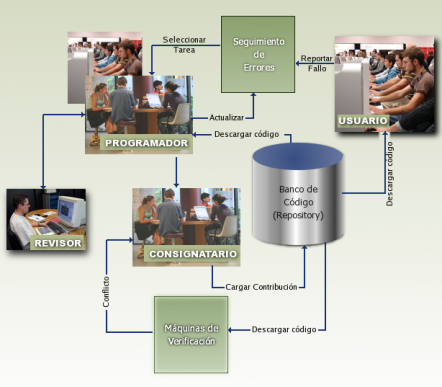
\includegraphics[width=100mm]{proceso_fs.png}
 \caption{Conceptos Básicos en el Desarrollo de Software de Código Abierto}
\label{proceso_fs} 
\end{figure}

Más que una forma de realizar sistemas, se trata de una visión revolucionaria en torno al software como patrimonio de la humanidad y se une a la filosofía del software libre que se expresa en \cite{stallman2002}:

\begin{quote}
“Software Libre” se refiere a la libertad de los usuarios para ejecutar, copiar, distribuir, estudiar, cambiar y mejorar el software. De modo más preciso, se refiere a cuatro libertades de los usuarios del software:

\begin{itemize}
\item La libertad de usar el programa, con cualquier propósito (libertad 0).
\item La libertad de estudiar cómo funciona el programa, y adaptarlo a tus necesidades (libertad 1). El acceso al código fuente es una condición previa para esto.
\item La libertad de distribuir copias, con lo que puedes ayudar a tu vecino (libertad 2).
\item La libertad de mejorar el programa y hacer públicas las mejoras a los demás, de modo que toda la comunidad se beneficie. (libertad 3). El acceso al código fuente es un requisito previo para esto.
\end{itemize}
\end{quote} 

Las aplicaciones más representativas del mundo del software libre como Apache, Mozilla, MySQL, PostgreSQL y el mismo sistema operativo Linux, luego de sus etapas primarias, adoptaron como proceso de desarrollo uno que contravenía en gran manera los fundamentos del control riguroso y ponía el futuro del sistema en manos de la anarquía \footnote{Definida en su sentido positivo como la situación humana en donde es innecesaria e indeseable la autoridad, lo que conlleva a una sociedad libre basada en el respeto mutuo de sus miembros y la cooperación voluntaria entre individuos.\cite{bce}}. Tal como lo propone Linus Torval “la idea es liberar versiones de prueba rápido a menudo, delegar cuanto sea posible, estar abierto hasta el punto de resultar promiscuo”.

Algunos principios fundamentales en este tipo de desarrollo los expone \cite{raymond}:

\begin{quote}
\begin{enumerate}
\item Todo buen trabajo de software comienza a partir de las necesidades personales del programador. (Todo buen trabajo empieza cuando uno tiene que rascarse su propia comezón). 

Esto podría sonar muy obvio: el viejo proverbio dice que "la necesidad es la madre de todos los inventos". Empero, hay muchos programadores de software que gastan sus días, a cambio de un salario, en programas que ni necesitan ni quieren. No ocurre lo mismo en el mundo Linux; lo que sirve para explicar por qué se da una calidad promedio de software tan alta en esa comunidad.
\item Los buenos programadores saben qué escribir. Los mejores, qué reescribir (y reutilizar).

... una importante característica de los grandes programadores es la meticulosidad con la que construyen. Saben que les pondrán diez no por el esfuerzo, sino por los resultados; y que casi siempre será más fácil partir de una buena solución parcial que de cero.
\item "Contemple desecharlo; de todos modos tendrá que hacerlo." cita encontrada en el capítulo 11 de libro The Mythical Man-Month escrito por el célebre Fred Brooks.

Diciéndolo de otro modo: no se entiende cabalmente un problema hasta que se implementa la primera solución. La siguiente vez quizás uno ya sepa lo suficiente para solucionarlo. Así que si quieres resolverlo, prepárate a empezar de nuevo al menos una vez.

\item Si tienes la actitud adecuada, encontrarás problemas interesantes.

\item Cuando se pierde el interés en un programa, el último deber es heredarlo a un sucesor competente.

\item. Tratar a los usuarios como colaboradores es la forma más apropiada de mejorar el código, y la más efectiva de depurarlo.

\item Libere rápido y a menudo, y escuche a sus clientes.

\item Dada una base suficiente de desarrolladores asistentes y beta-testers, casi cualquier problema puede ser caracterizado rápidamente, y su solución ser obvia al menos para alguien.

Dicho de manera menos formal, "con muchas miradas, todos los errores saltarán a la vista". A esto lo he bautizado como la Ley de Linus.

\item Las estructuras de datos inteligentes y el código burdo funcionan mucho mejor que en el caso inverso.

De nuevo Fred Brooks, Capítulo 11: “Muéstreme su código y esconda sus estructuras de datos, y continuaré intrigado. Muéstreme sus estructuras de datos y generalmente no necesitaré ver su código; resultará evidente.” 

\end{enumerate}
\end{quote} 
 
En general un proceso de desarrollo de software libre se basa en el hecho de que el programa puede ser instalado y el código fuente está disponible para cualquier persona. Es decir, la ausencia de barreras en cuanto a la limitación en el uso hace que muchas personas interesas en la funcionalidad que brinda el software lo descarguen y empiecen a utilizarlo. Dando inicio al siguiente ciclo:
\begin{enumerate}
\item El grupo inicial de programadores mantiene un sitio en la red para obtener retroalimentación de los usuarios los cuales reportan fallos, disafuncionalidades y solicitan nuevas características. 

\item Un desarrollador - que puede ser uno de los usuarios, revisa la lista de reportes y decide trabajar en uno específico; para tal efecto descarga la última versión del código fuente la modifica y la envía a un revisor para que este convalide la contribución.

\item La contribución se agrega al código fuente generando una nueva versión del sistema. Esto se realiza sincronizando el código fuente de desarrollo con aquél existente en la bodega de código fuente - repository, la cuál normalmente es un gestionada por un programa para el control de versiones. 

\item Si en algún momento dos programadores están realizando modificaciones a la misma porción de código y pretenden sincronizarlas ocurre un conflicto que deberá ser resuelto siguiendo reglas definidas que habitualmente contemplan el bloqueo de la versión más reciente, el aviso para resolución entre desarrolladores que causan el conflicto o el descarte de las contribuciones.
\end{enumerate}

De esta forma se va refinando el software siguiendo el ciclo mostrado en la figura \ref{proceso_fs}. El grupo de desarrollo se ve aumentado cuando usuarios expertos empiezan a proponer y realizar cambios directos en el código; cuando uno de ellos demuestra tener el suficiente interés y respeto hacia los intereses del software se le asigna el permiso para escribir directamente en la bodega de código.

La creación de la documentación así como de los modelos de requerimientos,análisis, diseño y despliegue siguen el mismo proceso.

\subsubsection{Métodos Ligeros}

Ha principios del milenio un grupo de experimentados desarrolladores, entre los que se encontraban Kent Beck, Alistair Cockburn, Martin Fowler y Dave Thomas, redactaron un manifiesto en el que consignaban los elementos de mayor importancia dentro del desarrollo de sistemas software \cite{beck1999}:
\begin{quote}
Nosotros estamos descubriendo mejores formas de desarrollar software dado que lo creamos y ayudamos a otros a realizar esta tarea. Por medio del trabajo de desarrollo hemos encontrado de gran valor elegir:

\begin{itemize}
\item \textbf{\textit{Individuos e interacciones}} sobre \textit{procesos y herramientas}
\item \textbf{\textit{Software ejecutable}} sobre \textit{documentación profusa}
\item \textbf{\textit{Colaboración del Cliente en el desarrollo}} sobre \textit{contrato de negocios}
\item \textbf{\textit{Respuesta al cambio}} sobre \textit{ceñirse a un plan.}
\end{itemize}

Mientras que existe valor en los elementos de la derecha nosotros valoramos más los elementos de la izquierda.\end{quote}

Con esto sentaban las bases para el despliegue de nuevos métodos de realizar software agrupados bajo el nombre genérico de “ágiles”\footnote{Siendo por definición un método caracterizado por ser liviano y ligero} que se contraponían a los métodos y procesos tradicionalmente rígidos y altamente planificados.

En \cite{koch} se expresan claramente las razones del porqué se desarrollan estos métodos y sus principales características. Los métodos ágiles nacen como respuesta del desarrollador puro al ambiente altamente industrializado y burocrático en el cual transcurren la mayoría de proyectos de desarrollo de software. En estos ambientes es típico el riguroso control que sobre el cumplimiento de cronogramas, planes de trabajo y presupuestos mantienen los denominados \textit{ingenieros de proceso}. El enfoque tradicional se basa en la planificación con la que se trata de \textit{predecir} desde las primeras etapas todos los pormenores del ciclo de desarrollo.

Debido a que los métodos tradicionales tienen fundamento en la ingeniería civil y mecánica, tratan de mitigar los riesgos poniendo un especial interés a las actividades de modelo en especial en las etapas de análisis y diseño; en general relegan a los desarrolladores a etapas de construcción erroneamente consideradas de \textit{cero esfuerzo} intelectual. Los requisitos del software se tratan de fijar desde los inicios del desarrollo, firmandose usualmente un contrato de aceptación de los mismos por parte del cliente. Estos métodos tradicionales siguen los lineamientos de aseguramiento de la calidad por la cual los procesos son eficientemente documentados, controlados, auditados, vigilados y mejorados. Todos esos aspectos hacen que el elemento clave sea el proceso y se relegue a segundo plano el crear productos que en realidad aporten un nuevo valor al cliente.

Para atacar la abrumadora complejidad que añade el proceso al sistema de software, los métodos ágiles proponen cambiar el paradigma \textit{predictivo} - rígido y resistente al cambio; por uno adaptativo que sea flexible y reaccione rápidamente antes cambios inesperados en los requisitos del software. Aquellos que han desarrollado un software de mediana o alta complejidad conocen de primera mano el hecho de que los requisitos no son estáticos, ellos cambian, evolucionan se transforman ya que en sí, no son sino abstracciones de necesidades del mundo real y este no es estático sino que se caracteriza por una fuerte dinámica.

El \textit{cliente también debe ser adaptable} en el sentido de que la mayoría de las veces los requerimientos del sistema los va descubriendo a medida que interactua con él. Una de las premisas de los procesos ágiles es el mantener un contacto permanente con el cliente e involucrarlo en todas las fases del desarrollo. Con esto se logra que el cliente obtenga un software que realmente cope sus intereses y (el cliente) sea consiente de los costos asociados al desarrollo del mismo.

Así como los requisitos cambian durante el desarrollo también lo hacen los recursos y el escenario en el cual se desenvuelve el equipo de trabajo. Para atacar esta característica de los sistemas software, se recomienda \textit{aferrarse a un presupuesto global} pero distribuyéndolo en pequeños presupuestos que solventen las tareas que ha corto plazo realizan los involucrados en el desarrollo.

Es claro con lo expuesto hasta ahora que el enfoque es considerar el desarrollo como una “\textit{carrera de 100 metros planos}” y no como una maratón. En tal sentido se deben gestar planes a corto plazo cuyo objetivo principal sea generar versiones del sistema que puedan ser probadas, corregidas e incrementalmente adicionadas en funcionalidad. Cada plan transcurre en lo que se denomina una iteración la cual usualmente no supera el mes de duración - algunos recomiendan una duración de dos semanas o ménos.\cite{beck1999}

Otro característica de los métodos clásicos, y que atacan los métodos ágiles, es aquella en la cual se considera a las personas como recursos intercambiables mediante la definición de \textit{roles} con funciones específicas y predictivas. Esto hace que las personas - cuyo comportamiento es poco predecible y no lineal \cite{cockburn1999}, tengan una moral baja y descienda su productividad; en el mejor de los casos trabajan con esfuerzo y, si sus condiciones son excelsas, rapidamente abandonan el grupo perdiéndose un activo intangible que repercute negativamente en la calidad global del sistema. Para los metodólogos ágiles el desarrollo se centra en las personas más que en los procesos, considera a cada miembro del grupo como un \textit{ser creativo e irreemplazable}, esto genera un gran cambio en cuanto al método: \textit{no es estático} ni recetario. Evoluciona, se recrea, se adapta y se concerta dentro el grupo de trabajo.

Evidentemente el proceso de desarrollo de software libre maneja los principios promulgados por los métodos ágiles los cuales encuentran quizás su máxima expresión en la Programación Extrema \cite{beck1999}.


\subsubsection{Proceso Unificado}
Según lo expresa \cite{alhir2003}:
\begin{quote}
El Proceso Unificado (UP) es un proceso de desarrollo de software basado en componentes dirigido por casos de uso, centrado en la arquitectura, iterativo e incremental...que utiliza la especificación UML dada por el Object Management Group (OMG) para preparar los esquemas del sistema. El Proceso Unificado es aplicable a diferentes tipos de sistemas de software, incluyendo proyectos de pequeña y larga escala; proyectos que tengan varios grados de complejidad técnica y administrativa, a través de diferentes dominios de aplicación y culturas organizacionales.

El PU nace de la unificación, en 1995, de la aproximación sugerida por Rational Software Corporation y el proceso orientado a objetos de la empresa Objetory AB. Se puede considerar al Proceso Unificado como un modelo de ciclo de vida del proyecto que incluye contexto, colaboraciones e interacciones. El UP es documentado totalmente en el libro “The Unified Software Development Process” escrito por Booch, Rumbaugh y Jacobson, y publicado por Addison- Wesley en 1999.\end{quote} 

Un sistema desde que nace hasta que muere repite el Proceso Unificado en ciclos de desarrollo constituidos por fases secuenciales cuyo objetivo es la producción incremental de liberaciones del sistema, llamadas comúnmente como generaciones del sistema. Cada una de las fases se convierte en un hito principal y esta constituido por pequeños microprocesos denominados \textit{iteraciones}. Habitualmente la numeración de las fases se hace de acuerdo a números enteros mientras que las iteraciones se hacen en números decimales. 

Las fases para el desarrollo de proyectos en el Proceso Unificado son cuatro \cite{jacobson2000}, a saber:

\begin{description}
\item [Fase de Concepción.] Tambien conocida como de inicio. Se centra en el establecimiento de las fronteras, ámbitos, riesgos asociados y visión del proyecto. Determina la viabilidad y los objetivos del proyecto. En esta fase podría tenerse una arquitectura general del sistema que esboze los subsistemas más importantes.

\item [Fase de Elaboración.] Se enfoca en la determinación de la arquitectura y requisitos del sistema; de esta forma se establece su viabilidad técnica. Durante esta fase se construyen los casos de uso críticos y se obtiene una arquitectura refinada del sistema. 

\item [Fase de Construcción] Es en la que se crea la mayor funcionalidad del producto, finaliza con cierta capacidad operativa. Se centra en la construcción del sistema y la arquitectura del sistema se considera estable.

\item [Fase de Transición]. Concluye con la liberación del producto, centrándose en la transición o distribución del sistema a la comunidad o usuario final. 

\end{description}

Dentro de las iteraciones el grupo de trabajo deberá distribuir sus esfuerzos en áreas estratégicas que conduzcan a la mitigación temprana de los riesgos, estás áreas son conocidas dentro del PU como disciplinas, figura \ref{proceso_unificado}:

\begin{itemize}
\item \textbf{Disciplina de administración de cambios en la configuración}, la cual se centra en la administración de la configuración del sistema y de las peticiones de cambios en la misma.

\item \textbf{Disciplina de administración de proyecto.}

\item \textbf{Disciplina de ambiente} que se centra en los ambientes de desarrollo del proyecto, incluyendo los procesos y las herramientas.

\item \textbf{Disciplina de modelado del negocio;} focalizado en la comprensión del negocio que esta siendo automatizado por el sistema capturando dicho conocimiento en un modelo del negocio.

\item \textbf{Disciplina de requerimientos,} necesaria para entender los requerimientos del sistema que automatiza el negocio y captura dichos requerimientos en un modelo de casos de uso.

\item \textbf{Disciplina de diseño y análisis,} centrada en analizar los requisitos y diseñar en sistema capturando tales  conocimientos en un modelo de análisis/diseño.

\item \textbf{Disciplina de implementación} para la implementación del sistema basado en el modelo de implementación.

\item \textbf{Disciplina de pruebas} que maneja las pruebas (evaluaciones) del sistema comparándolos con los requerimientos basándose primordialmente en el modelo de pruebas.

\item \textbf{Disciplina de distribución} encargada de la distribución del sistema basado en el modelo de distribución.
\end{itemize}

Durante la etapa de concepción la mayoría del esfuerzo está distribuido a través del modelo del negocio y la disciplina de requerimientos. 

Durante la fase de elaboración el esfuerzo se distribuye entre las disciplinas de implementación, diseño, análisis y requerimientos. Durante la etapa de construcción el esfuerzo se distribuye entre las disciplinas de análisis, diseño, implementación y pruebas. 

En la fase de transición el esfuerzo se distribuye a través de las disciplinas de prueba y distribución. Obviamente las disciplinas de soporte se distribuyen entre todas las cuatro fases. El objetivo general es producir el sistema, por lo tanto todas las disciplinas nucleares están comprometidas tanto como sea posible para no introducir riesgos en el proceso; esto es, los practicantes son los responsables de determinar cuales disciplinas comprometer y en que momento hacerlo.

En este punto es necesario definir varios conceptos: 
\begin{itemize}
\item \textbf{riesgo} en el Proceso Unificado se concibe como un obstáculo para alcanzar el éxito en la ejecución de una actividad, este riesgo puede estar determinado por características del negocio, humanas o técnicas.

\item \textbf{Iteración} es un paso o rama a través de un ruta hasta cierto destino. Dicho de otra forma es un movimiento planeado que puede ser evaluado para demostrar un progreso tangible dentro de una actividad o proceso, además, de acuerdo a lo citado por \cite{Zavala2000}: “Una iteración es iterativa en el aspecto de que es un acto repetitivo que propende la mejora continua del trabajo. Aditiva en el caso de que el resultado es siempre superior al alcanzado con un solo trabajo y paralela ya que el trabajo puede ser concurrente dentro de la iteración.”

\end{itemize}


\begin{figure}
 \centering
 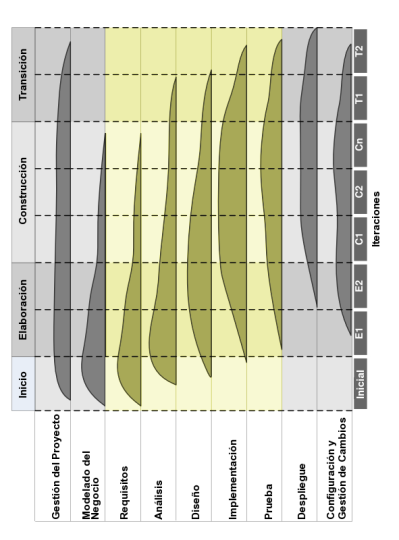
\includegraphics[width=140mm, height=190mm]{pu.png}
 \caption{Ciclo de Desarrollo de un sistema según el Proceso Unificado}
 \label{proceso_unificado}
\end{figure}

Cuando se decantan los \textit{requerimientos}, aquello que el sistema debe cumplir, se está declarando explícitamente los casos de uso los cuales, dado que el Proceso Unificado está manejado por ellos, determinan las iteraciones. De la misma forma en que los casos evolucionan en el marco de las disciplinas regidas por un proceso iterativo, los sistemas evolucionan constantemente con base en iteraciones realizados en el marco de su arquitectura. Incluyendo en la arquitectura todos los elementos, sus colaboraciones e interacciones.  

Resulta pues obvio que la iteración, dado que es un avance demostrable, tiende en últimas a reducir los riesgos inherentes a cada una de las etapas del proceso de desarrollo. Esto ha sido definido por \cite{alhir2003} en su artículo:
\begin{quote}
.. de esta forma las iteraciones confrontan los riesgos derivados de los casos de uso y la arquitectura para alcanzar el éxito en el proyecto, buscando en todo momento reconciliar las fuerza técnicas y del negocio. Una iteración esta acotada en el tiempo con inicio y final fijos en donde una colección de colaboraciones son planeadas, ejecutadas y evaluadas del tal forma que en todo momento se pueda demostrar progreso en el proceso... un caso de uso evoluciona a través de un gran número de iteraciones y a través de cualquier número de disciplinas nucleares en una iteración. La experiencia y aprendizaje obtenido en una iteración evidentemente conduce la aplicación de las próximas iteraciones dentro del proceso..\end{quote} 

La iteración se convierte en el hito más importante para asegurar el crecimiento continuo y el aseguramiento de la calidad total dentro del sistema que se está desarrollando. Las iteraciones marcan totalmente el ciclo de desarrollo del SITEM que utiliza una aproximación iterativa propuesta por el Proceso Unificado.

\section{UML: Lenguaje de Modelado Unificado}

Independiente del modelo utilizado para la construcción y gestión del desarrollo del sistema se requiere que la comunicación entre los diferentes integrantes del grupo de desarrollo sea efectiva. Se hace indispensable que todo el equipo utilice y entienda un lenguaje consistente y unificado con el cual expresen claramente sus ideas y desde el cual puedan marcar claramente las directrices a seguir. El lenguaje de Modelado Unificado, UML por sus siglas en inglés, brinda las características tanto sintácticas como semánticas para lograr caracterizar lógicamente cualquier tipo de software permitiendo ser utilizado en cualquier etapa del diseño y es especialmente útil en aquellos desarrollos enfocados a objetos.

El Lenguaje de Modelado Unificado es definido por el \textit{Object Management Group}\footnote{La página del OMG (www.omg.org) describe la organización como un consorcio de la industria de la informática, sin ánimo de lucro, con caracter internacional y de membresía abierta. Los diferentes grupos de trabajo del OMG desarrollan estándares en un rango amplio de tecnologías.}:
\begin{quote}
UML es un lenguaje visual para la especificación, construcción, y documentación de los artefactos de un sistema. Es un lenguaje de modelado de propósito generalque puede ser usado con la mayoría de los métodos orientados a objetos y a componentes; que puede ser aplicado a todos los dominios de aplicación (p.e., salud, finanzas, telecomunicaciones, aeroespacial) y plataformas de implementación (p.e., J2EE, .NET). \end{quote} 

En \cite{jacobson2005} se recalca que UML es usado para entender, diseñar, buscar, configurar, mantener y controlar la información acerca de los sistemas.

Con UML se crean artefactos con información acerca de la estructura - o vista estática- y el comportamiento - o vista dinámica- de un sistema. Cada vista del sistema se modela como una colección de objetos que interactuan, es decir, que tienen interfaces y relaciones entre ellos perfectamente definidas. Fruto de tal relación entre objetos el sistema ofrece una funcionalidad o cumple un objetivo que es de interés.
\section{Portales de Información y Conocimiento}

Antes de la explosión de servicios a través de la Internet, los portales basados en aplicaciones web estaban recomendados solo para organizaciones que por su complejidad (en tamaño ó geografía) necesitaran de un sistema tecnológico para que todo su personal pudiese tener acceso a la información en forma compartida y simultánea. Sin embargo, fundamentado en el crecimiento del uso de Internet\footnote{El porcentaje de la población con acceso a Internet en Colombia a crecido de un 2,1\% en el año 2000 a un 15,8\% en el 2007, según la Comisión de Regulación de Telecomunicaciones.} surgue la necesidad de la sociedad por mantener cierto orden en la corriente de bytes y grupos de usuarios con intereses de información comunes empiezan a conglomerarse alrededor de portales temáticos no organizacionales.

Un portal de información no es, en esencia, una fuente nueva de información; es una vista de la información existente que dispuesta en una forma ordenada se convierte en una herramienta de conocimiento extraordinariamente poderosa permitiendo poner al descubierto información valiosa que se enmascaraba entre otra no menos interesante – Data Mining.
Dentro de las múltiples ventajas que ofrece el portal, es que proporciona la facilidad de obtener información actualizada a muy corto plazo, lo que es indispensable para la óptima toma de decisiones. Dicha información esta disponible, en condiciones óptimas,  veinticuatro horas al día, trescientos sesenta y cinco días del año, permitiendo así acceder a los datos que se necesitan de acuerdo con la disponibilidad singular de tiempo y apoyar la toma de decisiones bajo cualquier circunstancia y lugar.

Gran cantidad de organizaciones y grupos de usuarios están explotando el uso de los portales creando y transformando servicios y procesos tradicionales convirtiéndolos en servidores de autoservicio, pudiendo así dedicarse a aquellos de mayor valor agregado a la organización, el personal o el grupo de investigación. 

\subsection{Beneficios y obstáculos para la implementación de portales basados en aplicaciones web.}

Las facilidades que proporciona la tecnología, permite que el portal sea accedido a través de numerosas opciones, esto es a través de computadoras de escritorio y portátiles integradas a la red interna de la organización, a través de Internet por redes de banda ancha y estrecha y de los diversos medios inalámbricos como son las tecnologías celular, WiFi, WiMax, BlueTooh por intermedio de PDA, celulares y equipos de cómputo en redes WLAN.

Debido a la estructura del portal, se tiene una fuerte correlación entre diversas aplicaciones que nos permiten analizar interrelaciones que serían realmente complejas y tardadas si no se contara con ellos. Sin embargo, es importante recalcar más que los beneficios los problemas potenciales. De hecho en el éxito de un portal están enfocados factores clave que tienen beneficios y problemas asociados.

\begin{description}
 \item[Factor Humano] Los individuos adaptan los procesos de información en diferentes maneras. 
 \item[Factor Tecnológico] Intranets, pueden ser costosas y poco efectivas si la organización no tiene la tecnología necesaria para construirlas.
 \end{description} 

La principal ventaja obtenida al construir y mantener un portal basado en aplicaciones web es mejorar la eficiencia y efectividad en la comunicación de los miembros de una organización o un grupo de usuarios, lo que aumenta la objetividad en la toma de decisiones y la transferencia de conocimiento. Todo lo anterior se maximiza si el portal se concibe como fruto de un proceso de investigación en donde todos sus componentes y servicios se construyen, mantienen, distribuyen e integran de acuerdo a los requerimientos de los usuarios finales\cite{sarmento2005}.

Una de las características importantes de los portales es que en un sólo lugar - y con un mecanismo de acceso unificado, los usuarios pueden acceder a las aplicaciones. Esta integración con aplicaciones y servicios orientados al trabajo colaborativo hacen que trascienda los límites de un mero repositorio organizacional - que permite el autoservicio de requerimientos y extracción de información básica - y lo convierte en una herramienta de administración del conocimiento, útil para la toma de decisiones.

Las novedosas tecnologías que convergen en Internet permiten que la información sea personalizada y dirigida de tal forma que se potencian ciclos de creación, captura y diseminación de conocimiento necesarios para el crecimiento de los activos intangibles de los grupos y organizaciones. Así los portales convierten la información en valor, ya que eliminan las barreras de distancia y disponibilidad de información, reduciendo costos conectando a múltiples personas en diversos sitios al mismo tiempo.

La tabla \ref{beneficio} muestra los principales beneficios potenciales de desplegar los portales de información y conocimiento dentro del quehacer de las organizaciones, los grupos de trabajo y las comunidades de práctica.

\begin{table}
\begin{center}
\begin{tabular}{|l|}
\hline
\textbf{Beneficios Humanos (suaves)}\\
\hline
Provee estructura de soporte 24 hrs.\\
Servicio centrado en el usuario.\\
Medio ambiente amigable.\\
\hline
\textbf{Beneficios Físicos y capitales (beneficios fuertes)}\\
\hline
Creación medioambiente libre de papel.\\
Mejorar eficiencia y efectividad.\\
Reducción de costos.\\
Menores tiempos en consecución de información.\\
\hline
\textbf{Beneficios estratégicos}\\
\hline
Creación de herramientas innovadoras de apoyo.\\
Proveer información a tiempo real.\\
Apoyo a proceso de negocios de reingeniería\\
Apoyo a los ciclos de creación, captura y diseminación de conocimiento.\\
Aumento de Capital intangible.\\
Formalización del \textit{Know-How}.\\
\hline
\end{tabular}
\caption{Algunos Beneficios Potenciales al Implementar un Portal}
\label{beneficio} 
\end{center}
\end{table}

Los riesgos que se afrontan también son enormes y pueden llevar al traste cualquier política o proyecto de desarrollo; la tabla \ref{riesgos} muestra algunos de los más importantes que deben ser minimizados.

\begin{table}
\begin{center}
\begin{tabular}{|l|}
\hline
\textbf{De tipo Humano (Fuertes)}\\
\hline
Indiferencia de la administración.\\
Sobrevaloración del papel de las TIC\\
Dirección centrada en el capital financiero\\
Estructuras organizacionales conservadoras.\\
Micropoderes y feudos organizacionales autogestionados.\\
Ignorancia y/o resistencia respecto al uso de TIC.\\
Resistencia a estandarizar la información.\\
Resistencia a compartir información/conocimiento.\\
\hline
\textbf{Riesgos Físicos/Capital}\\
\hline
Procesos orientados a la técnica y no multidimensionales.\\
Carencia de capital(TIC marginales).\\
Dificultad de integración de tecnología nueva y la existente.\\
Ausencia de inter, trans y multidisciplinariedad.\\
\hline
\textbf{Riesgos tecnológicos (Débiles)}\\
\hline
Estándares propietarios.\\
Redes de interconexión da baja velocidad.\\
Alta relación Consumo/Adopción de tecnología.\\
\hline
\end{tabular}
\caption{Algunos riesgos Potenciales al Implementar un Portal}
\label{riesgos} 
\end{center}
\end{table}

\subsection{Ciclo de Vida de los Portales}
Los portales como representación sistemática del quehacer de un grupo humano evoluciona en la medida que dicho grupo mejora su conocimiento de las relaciones entre sus miembros y el entorno que los rodean. En general pueden determinarse cinco macro-etapas~\cite{egovernment} que aumentan gradualmente su funcionalidad basado en el  conocimiento organizacional y la interrelación de usuarios a través del Portal:

\begin{description}
\item[Presencia Emergente]
Esta es la etapa primaria por la que pasa un portal en donde su funcionalidad es la de distribuir información interesante para un grupo de usuarios, el cual es totalmente caracterizado por el grupo de personas que construye - en todas sus dimensiones, el portal. Dichos usuarios no intervienen directamente en la estructura del Portal el cual complementa sus servicios por medio de enlaces y dependencia a otros portales temáticamente relacionados.

\item[Presencia Mejorada] 
Los usuarios pueden determinar en cierto grado la navegación a través de búsquedas en el archivo del sitio. Un portal en esta etapa presentará gran cantidad de información que usualmente se agrupa por áreas temáticas. Los mapas del portal se distribuyen profusamente con el fin de guiar a los usuarios en su tránsito por el mismo y usualmente un sistema básico de ayuda prediseñada esta disponible.
 
\item[Interacción]
Los portales registran a sus usuarios. Se implementan herramientas en línea como las salas de charla - chat, las listas de correo y los foros; se realiza capacitación básica por medio de seminarios basados en contenidos y se hace uso extensivo de recursos multimediales. La ayuda es síncrona o asíncrona pero ágil lo que fomenta una depuración y actualización de la información contenida en el portal.

\item[Transacción] 
Los usuarios realizan operaciones a través del portal. El comercio electrónico, la gestión de contenidos, la personalización de los ambientes del portal, búsquedas semánticas y el despliegue de servicios avanzados - cursos, blogs, etc; caracterizan esta etapa.

\item[Transformación] 
La etapa más avanzada de los portales en donde se han estructurado comunidades de práctica sobre temas concretos que potencian los ciclos de conocimiento mediante las herramientas brindadas por el portal. Se observa una jerarquía \textit{ad hoc} de usuarios con base en su aporte. Ellos mismos generan contenido que es convalidado por la comunidad y los administradores técnicos limitan sus funciones a aquellas relacionadas con mantener operativa la plataforma tecnológica. Las transacciones y el contacto en tiempo real son rutinarios. Las aplicaciones son de conocimiento general y el nivel de inmersión en el portal es alto.
\end{description}


\subsection{Aplicaciones Web}

También conocidas como \textbf{WebApps} son, en su concepción más básica, aplicaciones que responden a peticiones realizadas por un usuario por medio de un navegador (cliente) y ejecutan la lógica del programa en un servidor. Las aplicaciones web usualmente interactúan con sistemas de bases de datos y distribuyen los resultados de sus operaciones en lenguajes estándar tales como HTML, SMIL, XML,  RDF, SVG, etc.\cite{jackson2005}. Las WebApps también se pueden encontrar en ambientes diferentes al modelo cliente - servidor\cite{bos2004}. 

Entre las características de las aplicaciones web se destacan\cite{bos2004}:

\begin{itemize}
\item \textbf{No requieren instalación.} En general las aplicaciones web no necesitan ejecutar rutinas de instalación en las máquinas cliente. Quizás en algunos lenguajes sea necesario la preparación de un ambiente específico de trabajo que en la mayoría de las veces es de acceso público.

\item \textbf{Accesibilidad.} Las aplicaciones web se despliegan desde de una página web. Los protocolos usados son estandarizados y abstraen fácilmente las capas de aplicación de las de diseño y datos.

\item \textbf{Facilidad en el Desarrollo.} Los lenguajes usados son de alto nivel, con un buen soporte para cadenas de caracteres, diferentes tipos de datos y con facilidades para la programación orientada a objetos. La mayoría de ellos con sintaxis similares y herramientas de desarrollo gratuitas de fácil adquisición. 

\item \textbf{Independencia de la Plataforma.} Las \textit{WebApps engines} implementan el modelo de capa intermedia lo que permite que las diferentes WebApps puedan ser desplegadas sobre diferentes plataformas sin detrimento de su funcionalidad. El uso de métodos genéricos definidos en interfaces de programación (API) ayuda en gran manera a garantizar esta característica.

\item \textbf{Seguridad.} No obstante la facilidad de acceso de la WebApp, estas pueden implementar rutinas avanzadas que brindan ambientes transaccionales seguros aislados del sistema de archivos y configuración del sistema en donde se alojan. El intercambio de información cifrada por la red y la integración con la seguridad de los servidores de bases de datos forman un contexto de alta seguridad.

\item \textbf{Privacidad.} Las WebApps pueden operar fácilmente sobre una Plataforma de Preferencias de Privacidad debido a que la mayoría de los motores están habilitados para soportar el protocolo \textbf{P3P}.

\item \textbf{Almacenamiento Persistente.} Tanto en el cliente - a través de archivos texto para el manejo de sesiones; como en el servidor de base de datos.

\item \textbf{Integración.} Las aplicaciones Web pueden brindar sus servicios - u obtener uno determinado, a través de interfaces claras y definidas en las denominadas redes de servicios Web.
\end{itemize}

\section{Aspectos Claves en la Gestión y Dirección del Conocimiento}

Como se aclaró anteriormente, OpenSITEM es una federación de diferentes tipos de sistemas software y sirve de soporte para el trabajo de los equipos de diseño de redes de eSalud del grupo de investigación GITEM (o similares). En esa línea, parte de su funcionalidad está enfocada en brindar apoyo a los flujos de trabajo de comunidades de práctica yu por tanto es necesario que se aborden aspectos relacionados con la gestión del conocimiento. A continuación se presenta la aproximación conceptual de está área.

\subsection{Acerca del conocimiento}

En la presente investigación conocimiento es entendido como un concepto que encierra, entre otras, las siguientes definiciones y se usarán de acuerdo a su contexto como partes complementarias de una misma meta – definición.

De acuerdo con Gunter Dueck\cite{dueck2001}, el conocimiento es un concepto que puede tener componentes en una o varias de las siguientes dimensiones:

\begin{itemize}
\item  \textbf{Episteme} -\textit{ Dimensión abstracta – o metafísica}, en forma de generalizaciones, bases, leyes y principios científicos.

\item \textbf{Phronesis }– \textit{Dimensión práctica}, relativa al conocimiento pragmático discernido a través de las practicas aceptadas por la sociedad.

\item \textbf{Techne} – \textit{Dimensión técnica}, relativa a la forma de hacer las cosas, de la realización de actividades concretada en la forma de manuales, procedimientos y comunidades de práctica.

\item \textbf{Metis} – \textit{Dimensión objetiva}, como forma de volver corpóreo, real y sustancial la conjugación de los otros tipos de conocimiento.
\end{itemize}

Esta concepción multidimensional extiende y explica la taxonomía del conocimiento dada por los griegos:

“El conocimiento incluye restricciones implícitas y explícitas entre objetos (entidades), operaciones y relaciones, que permiten recoger heurísticas generales y específicas así como los procedimientos de inferencias relacionados con la situación a modelar”.\cite{sowa1984}

Otros autores despojan del sentido filosófico y colocan su definición en un plano simple y utilitario: “El conocimiento es información organizada y analizada para hacerla comprensible y aplicable a la resolución de problemas y toma de decisiones”.\cite{turban1992}. Si bien esta es una definición reduccionista, sirve de base para las propuestas de representación de conocimiento en documentos XML - comúnmente denominadas \textit{ontologías}. 


\subsection{Ciclo de Conocimiento}

Múltiples factores deben ser considerados cuando se trata de capturar, crear y diseminar el conocimiento dentro de un grupo de personas. La no homogeneidad en los medios de almacenamiento de conocimiento es uno de ellos. El conocimiento - en cualquiera de sus formas, puede estar guardado en diferentes partes que van desde entidades biológicas - mente humana, genes; a repositorios de conocimiento estructurado tales como ontologías, grafos de relación o mapas mentales.

Otro factor importante es la capacidad de acceso al conocimiento que es muy diferente al mero hecho de acceder a una fuente de conocimiento dada. En \cite{nokata1995} se considera que el conocimiento puede estar en dos estadios con propiedades diferentes: tácito y explícito. 

\begin{itemize}
\item \textbf{Conocimiento tácito:} Este conocimiento se corresponde con el conocimiento obtenido a través de la experiencia, conocimiento simultáneo  y conocimiento análogo. Esta forma de conocimiento usualmente se encuentra en medios de almacenamiento biológicos como la mente humana.

\item \textbf{Conocimiento explícito:} Se corresponde con el conocimiento racional, conocimiento secuencial, y conocimiento digital y se encuentra almacenado en documentos, bases de conocimiento, ontologías o cualquier otro medio abstracto de representación.
\end{itemize}

En \cite{liebowitz1998} se establece un tercer estadio llamado conocimiento implícito.

\begin{itemize}
\item \textit{Conocimiento Implícito:} Acceso directo mediante consulta y discusión. Requiere la localización y comunicación previa de conocimiento informal.
\end{itemize}

Un \textit{Ciclo de Conocimiento} es el proceso por el cual el conocimiento se transforma de tácito a explícito y viceversa por medio de las siguientes actividades:

\begin{itemize}
\item \textbf{Socialización:} Compartir conocimiento tácito entre individuos. El conocimiento permanece siendo tácito sin ser transformado en explícito. Este tipo de patrón no es muy interesante debido a su naturaleza tácita (Tácito - Tácito).

\item \textbf{Articulación:} Alguien transforma el conocimiento tácito en explícito (Tácito - Explícito).

\item \textbf{Síntesis:} Combinación de conocimiento explícito para crear nuevo conocimiento explícito  (Explícito - Explícito).
 
\item \textbf{Interiorización:} Proceso de transformar conocimiento explícito en tácito (Explícito - Tácito).
\end{itemize}

\begin{figure}
 \centering
 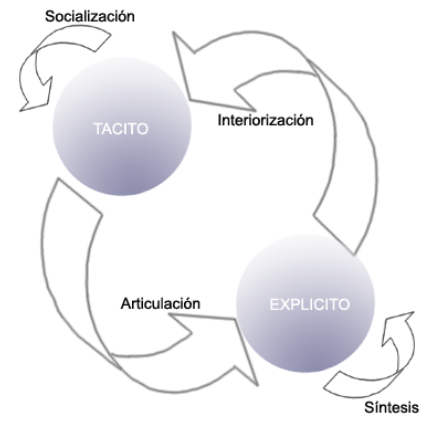
\includegraphics[width=100mm]{Ciclo_Conocimiento.png}
 \caption{Ciclo de Conocimiento}
 \label{ciclo_conocimiento}
\end{figure}

El flujo de conocimiento organizacional más importante es la transformación del conocimiento tácito en explícito \cite{davies2011}, esto es, la \textit{articulación} que se apoya en procesos avanzados de socialización. Esto permite acumular conocimiento explícito que puede ser compartido y accedido por los miembros de la organización. Por el contrario, la interiorización es el proceso natural llevado a cabo a través del aprendizaje individual por parte de los integrantes de la organización, esto es, la asimilación de conocimiento. 

El tercer flujo de conocimiento relacionado con la transformación de conocimiento es la \textit{combinación} o síntesis. En este caso se transfiere conocimiento a otra forma explícita de conocimiento. Un ejemplo sería el cambiar el formato de una base de conocimiento, agrupar ontologías o refinar heurísticas. Este tipo de flujo de conocimiento es importante para seleccionar, combinar y distribuir el conocimiento existente con diferentes fines. Por ser quizás el flujo de conocimiento más formal en OpenSITEM algunos componentes específicos implementan flujos de síntesis de conocimiento.

El cuarto flujo del ciclo de vida del conocimiento permite transformar conocimiento tácito en otras formas de conocimiento tácito mediante procesos de socialización. Un ejemplo de esto es cuando se transfiere conocimiento tácito de un experto a un ingeniero de conocimiento en una entrevista personal.

\subsection{Tecnologías del Conocimiento}

En la actualidad el conocimiento se considera un activo fundamental y como lo expresa \cite{gang2007}, tiene dos propiedades de vital importancia para contribuir al desarrollo de las organizaciones o comunidades de práctica:

\begin{itemize}
\item \textbf{Es explicable.} Cuando no se evidencia esta propiedad el conocimiento permanece tácito y en ninguna medida puede considerarse como perteneciente a la comunidad o la organización. Es entonces una tésis que solo aquel conocimiento que se ha convertido en explícito es el que posee una organización; de otra manera es propiedad exclusiva del individuo.

\item \textbf{Se puede comunicar y compartir.} Cuando no se toman medidas que formalicen estas actividades el conocimiento se pierde. Es decir, la organización o comunidad debe tener procesos conocidos que garanticen flujos de conocimiento basados en la síntesis, interiorización y socialización.
\end{itemize}

En general para que el conocimiento pueda generar ventajas competitivas debe ser gestionado de alguna manera. Esta necesidad dio surgimiento a dos áreas de investigacion comunmente agrupadas bajo el concepto de Tecnologías de Conocimento: Ingeniería de Conocimiento y Gestión de Conocimiento. 

Uno de los primeros problemas que deben atacar las tecnologías de conocimiento es el asociado con el Modelado de Conocimiento. En \cite{benafia2016} se expresan algunos principios a tener en cuenta cuando se modela el conocimiento:

\begin{itemize}
\item \textbf{Definición de roles de conocimiento}. El conocimiento se puede dividir en unidades atómicas que tienen propiedades irreductibles y que se asocian para lograr funciones que identifican dicha unidad.

\item \textbf{Identificación de tipos de conocimiento.} Cada unidad de conocimiento debe enmarcarse en uno o varios de los siguientes tipos de conocimiento: de tareas, inferencial, del dominio, ontologías del dominio, modelos del dominio. 

\item \textbf{Capacidad de ser compartido y reutilizado.} Las unidades de conocimiento pueden ser expresadas usando lenguajes y reglas formales. Lo que permite que pueda ser entendido por entidades con roles de conocimiento definidos.

\item \textbf{Uso de modelos gráficos.} La unidades de conocimiento pueden ser representadas mediante grafos tipo red en los cuales tanto los nodos como las rutas de interconexión son unidades atómicas de conocimiento.
\end{itemize}


\subsection{Gestión de conocimiento}

La gestión del conocimiento es de esos conceptos \textit{polisémicos} que no pocos autores pretenden consolidar en una sola definición \cite{girard2015}. En este proyecto partimos de una visión sistémica que lo transcienda a lo que en investigación holística se comprende como sintagma\cite{hurtado2000}. La \textit{gestión de conocimiento}, como se percibe en la presente investigación, es “una unión sintagmática de diversos paradigmas” \cite{hurtado2000}. Fue \textit{Karl Wiig}, quien usó el término de \textit{gestión de conocimiento} por primera vez durante una conferencia en Suiza y a partir de ese momento diversos autores han conceptualizado el término surgiendo definiciones parciales tales como:

“La Gestión de Conocimiento es la construcción y aplicación sistemática, explícita y deliberada de conocimiento para maximizar la efectividad organizacional con respecto al conocimiento, por lo que usa sus activos de conocimiento”\cite{wiig1993}

“La Gestión de Conocimiento es el proceso de capturar experiencia colectiva organizacional donde ésta resida (por ejemplo, bases de datos, documentos, mentes humanas) y su distribución allá donde pueda ayudar a mejorar los resultados”\cite{hibbard1997}

“La Gestión de Conocimiento es la gestión y control explícito del conocimiento en una organización para lograr los objetivos de la organización” (van der Spek and Spijkervet, 1997)

Consecuente con la concepción de la gestión de conocimiento como un sintagma se puede concebir un paradigma asociado a un proceso con ciertas actividades implicadas: 

\begin{itemize}
\item Identificación y mapeo de bienes intelectuales de la organización.
\item Generación de conocimiento nuevo que permita obtener una ventaja competitiva. 
\item Recopilación accesible de información organizacional. 
\item Compartir buenas prácticas y tecnología, incluyendo técnicas de trabajo en grupo.
\end{itemize}

Este paradigma explora el conocimiento técnico, pragmático y objetivo considerando que la conjugación de leyes rígida e epistemológicas van en contravía de la dinámica misma de los sistemas. La articulación de este conocimiento debe ser mantenido de alguna forma en la organización, y de ahí surge el concepto de Memoria Corporativa. El saber hacer está completamente diseminado en la organización y debe ser integrado de forma coherente para facilitar el acceso al mismo y su reutilización, esto es, expresarlo en forma de memoria corporativa. 

Las memorias corporativas se consideran un elemento clave para gestionar el conocimiento porque facilitan su conservación, distribución y reutilización. Van Heijst define la memoria corporativa como una “representación de conocimiento e información organizacional explícita y persistente”, mientras que en (Nagenda y Plaza, 1996) se define como “los recursos colectivos de datos y conocimiento de una compañía, incluyendo experiencias en proyectos, experiencia en resolución de problemas, etc”. En (Abecker, 1998), una memoria corporativa es referida como “un contenedor que integra información contextual, documentos e información no estructurada, que facilita su uso y reutilización”.

%\section {Ontologias}


1.5 ONTOLOGÍAS

Tal como ocurre con el conocimiento, el concepto de ontología ha recibido múltiples definiciones a lo largo de la historia y es necesario aclarar que, una vez más y debido a sus múltiples usos, el término trasciende sus raíces etimológicas y filosóficas para convertirse en si mismo en un concepto con semántica de tipo contextual. Inicialmente para la filosofía una ontología es una 
“Parte de la metafísica que trata del ser en general y de sus propiedades trascendentales.” Diccionario de la Real Academia de la Lengua

“Ciencia o estudio del ser: específicamente, una rama de la metafísica relacionada con la naturaleza y las relaciones del ser; un sistema particular según el cual se investigan los problemas de la naturaleza del ser; esto es, filosofía fundamental”.

“Teoría relativa a los tipos de entidades y específicamente los tipos de entidades abstractas que se admiten en el lenguaje de un sistema” 

Q!ueda claro que el término ha sido tomado prestado de ls escuales filosóficas y es por ende allí en donde se puede obtener un contexto más apropiado que pèrmita concretar lo que, en el campo de la gestión de conocimiento, una ontología pretende englobar.

La “Oxford Companion of Philosophy” define ontología de la siguiente forma: 

 “Ontología, entendida como una rama de la metafísica, es la ciencia del ser en general,       abarcando aspectos como la naturaleza de la existencia y la estructura categórica de la       realidad. El término ontología tiene algunos usos adicionales en filosofía. En un sentido       derivativo se usa para referirse a un conjunto de cosas cuya existencia queda reconocida por una teoría o sistema de pensamiento. En este sentido se habla de la ontología de una teoría o de un sistema metafísico definido por tal ontología”

Y es por esto que la ontología puede ser concebida como una forma de reconocer – formalizar, la existencia de supuestos metafísicos tales como el conocimiento. Es esta formulación la que comúnmente es aceptada en el área de la inteligencia artificial sobre todo la expresada por Quine (Quine, 1961), quien dijo que todo lo que puede ser cuantificado existe.

La primera definición de ontología en Inteligencia Artificial apareció en (Neches et al, 1991):

“Una ontología define los términos básicos y relaciones que conforman el vocabulario de un área específica, así como las reglas para combinar dichos términos y las  relaciones para definir extensiones de vocabularios”

Una de las definiciones más extendidas es la dada por Tom Gruber (Gruber, 1993): 

 "Una ontología es una especificación explícita de una conceptualización. El término       proviene de la filosofía, donde una ontología es un recuento sistemático de la existencia. En sistemas de Inteligencia Artificial, lo que existe es lo que puede ser representado. Cuando el conocimiento de un dominio se representa mediante un formalismo declarativo, el conjunto de objetos que puede ser representado se llama universo del discurso. Esos conjuntos de objetos, y las relaciones que se establecen entre ellos, son reflejados en un vocabulario con el cual representamos el conocimiento en un sistema basado en conocimiento. Así, en el contexto de IA, podemos describir la ontología de un programa como un conjunto de términos. En tal ontología, las definiciones asocian nombres de entidades del universo del discurso con textos comprensibles por los humanos que describen el significado de los nombres, y axiomas formales que limitan la interpretación y buen uso de dichos términos. Formalmente, una ontología es una teoría lógica”
     
Gruber entiende por conceptualización “una interpretación estructurada de una parte del mundo que usan los seres humanos para pensar y comunicar sobre ella. Para un informático, una conceptualización podría ser la clasificación de sistemas informáticos atendiendo a su naturaleza física en sistemas hardware, sistemas software y sistemas firmware.” (Fernández, 2003). Además dicha conceptualización debe ser, de alguna forma, factible de ser compartida y entendida.

Nicola Guarino (Guarino, 1995) tratando de crear una definición concertada  expresó:

“Un punto de inicio en este esfuerzo clarificador será el cuidadoso análisis de la       interpretación dada por Gruber. El problema principal de dicha interpretación es que se basa en la noción de conceptualización. Una conceptualización es un conjunto de relaciones extensionales que describen un estado particular, mientras que la noción que tenemos en mente es intensional, esto es, algo como una rejilla conceptual al que le imponemos varios posibles estados ...En el sentido filosófico, podemos referirnos a una ontología como un sistema particular de categorías que representa una cierta visión del mundo. Como tal, este sistema no        depende de un lenguaje particular: la ontología de Aristóteles es siempre la misma,       independientemente del lenguaje usado para describirla. Por otro lado, en su uso más típico en IA, una ontología es un artefacto ingenieril constituido por un vocabulario específico para describir una cierta realidad, más un conjunto de supuestos explícitos concernientes al significado pretendido de las palabras del vocabulario. Este conjunto de supuestos tiene generalmente la forma de teorías lógicas de primer orden, donde las palabras del vocabulario aparecen como predicados unarios o binarios, respectivamente llamados conceptos y relaciones. En el caso más simple, una ontología describe una jerarquía de conceptos relacionados por relaciones de subsunción; en los casos más sofisticados, se añaden axiomas para expresar otras relaciones entre conceptos y restringir la posible interpretación.”

Más tarde Guarino modificaría su definición para abarcar conceptos más globales para la interpretación afirmando que: 

“Una ontología puede especificar una conceptualización en una forma muy indirecta, puesto que i) solo puede aproximar un conjunto de modelos pretendidos; y ii) tal conjunto de modelos pretendidos sólo es una caracterización débil de una conceptualización.”. (Guarino, 1998)

Borst (Borst, 1997), redefine la ontología de Gruber:

“Una ontología es una especificación formal de una conceptualización compartida.” 

A la par que (Studer et al, 1998) explica que:
“Conceptualización se refiere a un modelo abstracto de algún fenómeno en el mundo a través de la identificación de los conceptos relevantes de dicho fenómeno. Explícita significa que el tipo de conceptos y restricciones usados se definen explícitamente. Formal representa el hecho de que la ontología debería ser entendible por las máquinas. Compartida refleja la noción de que una ontología captura conocimiento consensual, esto es, que no es de un individuo, sino que es aceptado por un grupo” 

Con lo anterior se puede tener una visión adecuada de las ontologías – quizás no completa pero práctica, que permite asociar técnicas a la definición propia de estructuras que modelen y sirvan para expresar – socializar, el estado de conceptos abstractos.

1.5.1 Tipos de ontologías
      
En general las ontologías, referidas como medio para modelar sistemas abstractos, pueden ser clasificadas de acuerdo a ciertos criterios como son: (a) el tipo de conocimiento contenido; y (b) la motivación de la ontología.

1.5.1.1. Ontologías según el conocimiento contenido

Este es el criterio donde existe mayor diversidad, la cual puede ser ilustrada por las dos siguientes clasificaciones de ontologías. La primera de ellas fue propuesta en (Van Heijst et al, 1997), donde se distinguen tres tipos de ontologías: 
Ontologías terminológicas, lingüísticas: Especifican los términos usados para representar conocimiento en el dominio. Un ejemplo de este tipo de ontologías es la red semántica UMLS (Unified Medical Language System) (Lindberg et al, 1993).

Ontologías de información: Especifican la estructura de los registros de la base de datos. Los esquemas de bases de datos serían un ejemplo. 

Ontologías para modelar conocimiento: Especifican conceptualizaciones de conocimiento. Estas ontologías tienen una estructura interna mucho más rica que los anteriores tipos de ontologías, y éstas son las ontologías que interesan a los desarrolladores de sistemas basados en conocimiento.      

Una clasificación alternativa fue propuesta en (Mizoguchi et al, 1995), donde también se proponen tres categorías:

Ontologías del dominio: Contienen todos los conceptos asociados a un dominio particular.
Ontologías de tarea: Establecen la forma en la cual se puede usar el conocimiento del dominio para realizar tareas específicas. De esta forma, una aplicación podría realizar búsquedas de información mientras otra podría gestionar la asignación de bloques libre de memoria.
Ontologías generales: Contienen descripciones generales sobre objetos, eventos, relaciones    temporales,   relaciones    causales, modelos de  comportamiento y funcionalidades.

1.5.1.2. Ontologías por motivación para su creación

Inicialmente se distinguen cuatro tipos de ontologías:

Ontologías para la representación de conocimiento: Permiten explicar las conceptualizaciones que subyacen de los formalismos de representación de conocimiento (Davis et al, 1993).

Ontologías genéricas: Definen conceptos considerados genéricos en diferentes áreas. Ejemplos de tales conceptos serían componente, subclase, proceso, estado, etc. Estas ontologías son reutilizables en diferentes dominios. Se llaman también ontologías abstractas o superteorías porque permiten definir conceptos abstractos, y dichas ontologías pueden ser usadas para definir conceptos de forma más específica en diferentes dominios. Como ejemplos podemos ver la taxonomía, la mereología, la topología y la teoría general de sistemas.

Ontologías del dominio: Definen conceptualizaciones específicas del dominio. Las metodologías actuales de adquisición de conocimiento distinguen entre ontologías y conocimiento del dominio, porque el último describe situaciones factuales del dominio, mientras que las ontologías imponen descripciones sobre la estructura y contenido del conocimiento del dominio.

Ontologías de aplicación: Están ligadas al desarrollo de una aplicación concreta. Tales ontologías cubren los aspectos relacionados con aplicaciones particulares. Típicamente, estas ontologías toman conceptos de ontologías del dominio y genéricas, así como métodos específicos para realizar la tarea, por lo que no son muy adecuadas para ser reutilizadas.

Una clasificación alternativa fue propuesta por Poli (Poli, 2000). En dicha clasificación se identifican los siguientes tipos de ontologías: 

Ontologías generales: Tienen que ver con las categorías fundamentales y sus conexiones de dependencia. Con respecto a las categorías fundamentales, los investigadores se dan cada vez más cuenta de la dificultad de manejar este nivel supremo. Por ello, es de máxima importancia emplear una organización de categorías principales que sea lo más transparente posible. Existen categorías fundamentales que se aplican a todos los niveles ontológicos. Sin embargo, muchas de las categorías top- level pueden tener diferentes valores en niveles diferentes de la ontología, aunque deben  tener algo en común. 

Ontologías categóricas: Estudian las diversas formas en las que una categoría se da cuenta de los diversos niveles ontológicos, determinando la posible presencia de una teoría general que subsume sus concretizaciones. Mientras que la ontología general está más relacionada con la arquitectura de la teoría, la ontología categórica es más sensible a los detalles de las categorías individuales. Sin embargo, es obvio que ambas son necesarias.

Ontologías del dominio: Se refieren a la estructuración detallada de un contexto de análisis con respecto a los subdominios que lo componen. 

Ontologías genéricas: Parecen ligadas a corpus lingüísticos y léxicos conceptuales. De hecho, se pueden clasificar los términos en varios niveles. Esto significa que cada término debería ser accesible por defecto únicamente en su sentido genérico, mientas que sus significados especializados quedan para cuando se active una ontología del dominio específica. Por otro lado, la ontología del dominio contiene términos que no tienen correspondencias analíticas en ontologías genéricas. El conocimiento del dominio “satura” el conocimiento genérico.

Ontología regional: Analiza las categorías y sus conexiones de interdependencia para cada nivel ontológico (estrato o capa). 

Ontología aplicada: Estas ontologías son la aplicación concreta de entorno ontológico a un objeto específico (por ejemplo, un proyecto).

 1.5.2. Ontologías de tipo Formal y Descriptiva

Una tercera clasificación se basa en el grado de formalidad de la ontología. Según este criterio se distinguen tres tipos de ontologías en (Poli, 2002): 

Ontología descriptiva, relacionada con la recolección de información sobre los ítems del dominio analizado. La unidad y variedad del mundo es la salida de las conexiones de dependencia y formas de independencia entre los ítems. Cosas materiales, plantas y animales, así como los productos de los talentos y actividades de animales y humanos, son ítems del mundo. 

En otras palabras, el mundo no solo contiene cosas, animadas o no, sino también actividades y procesos, así como los productos derivados de los mismos. Es difícil negar que existen pensamientos, sensaciones y decisiones, así como el completo espectro de actividades mentales, así como uno está obligado a admitir la existencia de reglas, lenguajes, sociedades y costumbres (Poli,2001a).        

Ontología formal, que destila, filtra, codifica y organiza los resultados de una ontología descriptiva. Según esta interpretación, la ontología formal es formal en el sentido usado por Husserl es sus “Logical Investigations”. Ser formal en este sentido implica tratar con categorías como cosa, proceso, materia, forma, todo, parte, etc. Estas categorías caracterizan aspectos y tipos de realidad que todavía no han sido utilizados bajo ningún formalismo.        

La codificación formal en sentido estricto se da al nivel de ontología formalizada. El objetivo es encontrar la codificación formal apropiada para los constructores adquiridos de forma descriptiva y purificarlos formalmente como se indica. El nivel de construcciones formalizadas también está relacionado con la evaluación de la adecuación (expresiva, computacional, cognitiva) de los distintos formalismos, y con el problema de las traducciones recíprocas. La fuerte similaridad entre los términos “formal” y “formalizada” es un contratiempo. Una forma de evitar la confusión es utilizar “categórica” en vez de formal. La mayor parte de las teorías contemporáneas sólo reconocen dos niveles de análisis y suelen unir las categorías formales con el análisis formalizado. Como consecuencia, se suele negar la relevancia específica de los análisis categóricos. 

Los tres niveles ontológicos son diferentes pero no están separados, puesto que están relacionados en muchos aspectos. El conocimiento descriptivo puede referirse a categorías formales, y las salidas formalizadas a los otros dos niveles. Por otro lado, es más delicado establecer las diferencias y conexiones entre varias facetas ontológicas como se muestra en (Poli, 2002a).        

La aplicación de métodos lógico-formales a una ontología la transforma en ontología formal. Los primeros ontólogos formales creían que la tarea de construcción podía ser llevada a cabo de forma sistemática y está completamente basada en la resolución de problemas lógicos, esto es, en la gramática lógica de lenguajes particulares. En contraste, la antigua tradición ontológica se ha quedado en un almacén de intuiciones ontológicas, constituyendo argumentos informales e incluso retóricos sobre esas intuiciones como base. Como se establece en (Gangemi et al, 1999),       las relaciones formales implican entidades de todas las esferas materiales, de forma que son comprensibles per se como nociones universales. Por el contrario, las relaciones materiales son específicas de una o más esferas materiales. Esto presupone una división a priori del dominio en esferas materiales: primero se debe realizar una distinción entre relaciones formales y materiales con base a su comportamiento con respecto a tales subdominios. De esta forma, las relaciones formales establecen las conexiones y las diferencias entre subdominios primitivos, mientras que las relaciones materiales caracterizan las propiedades de un subdominio específico. Si se asume un dominio plano, sin estructura a priori, entonces no sería válida la distinción entre relaciones formales y materiales. 

1.5.3 Ingeniería Ontológica

Las ontologías proporcionan un vocabulario común de un área y definen, a diferentes niveles de formalismo, el significado de los términos y relaciones entre ellos. El conocimiento en ontologías se formaliza principalmente usando cinco tipos de componentes: clases, relaciones, funciones, axiomas e instancias (Gruber, 93).

Las clases en la ontología se suelen organizar en taxonomías. Algunas veces, la noción de ontología se diluye en el sentido que las taxonomías se consideran ontologías completas [Studer et al.; 98]. Se suele usar tanto el término clases como conceptos. Un concepto puede ser algo sobre lo que se dice algo y, por lo tanto, también podría ser la descripción de una tarea, función, acción, estrategia, proceso de razonamiento, etc. 

Las relaciones representan un tipo de interacción entre los conceptos del dominio. Se definen formalmente como cualquier subconjunto de un producto de n conjuntos, esto es: 
R: C1 x C2 x ... x Cn.
Como ejemplos de relaciones binarios incluimos: “subclase de” y “conectado a”. Las funciones son un tipo especial de relaciones en las que el n-ésimo elemento de la relación es único para los n-1 precedentes. Formalmente, definimos las funciones F como: 
F: C1 x C2 x ... x Cn-1 x  Cn. 
Como ejemplos podemos mencionar las funciones “madre de” y “precio de un coche usado”. 

Los axiomas son expresiones que son siempre ciertas. Pueden ser incluidas en una ontología con muchos propósitos, tales como definir el significado de los componentes ontológicos, definir restricciones complejas sobre los valores de los atributos, argumentos de relaciones, etc verificando la corrección de la información especificada en la ontología o deduciendo nueva información. Tales ontologías son llamadas ontologías pesadas, en contraste con las ontologías ligeras que no incluyen axiomas. 

Las instancias se usan para representar elementos específicos.

1.5.3.1. Relaciones

En (Gómez-Pérez et al, 2000) se enumeran las relaciones más comunes en dominios reales, a saber: equivalencia, taxonómica, partonómica, dependencia, topológica, causal, funcional, cronológica, similaridad, condicional y propósito. Sin embargo, no todas las relaciones tienen la misma relevancia ni imponen el mismo tipo de propiedades jerárquicas a la ontología. Entre este conjunto de relaciones podemos subrayar tres de ellas: taxonomía, mereología, y topología. Taxonomía.

La palabra taxonomía tiene su origen en dos términos griegos, a saber, taxis (orden) y nomos (tratado) y esta palabra proviene de la Filosofía. Taxonomía es la ciencia que estudia la división en grupos ordenados o categorías. Desde un punto de vista ontológico, una taxonomía es una organización ontológica basada en una relación de orden parcial llamada IS-A, a través de la cual se agrupan las entidades y son subsumidas por clases de más ato nivel. En general, las taxonomías han sido importantes para modelar esquemas de bases de datos, sistemas basadas en
conocimiento y vocabularios semánticos (Guarino and Welty, 2001).

A continuación se presentan las propiedades satisfechas por las relaciones taxonómicas. Con este propósito, se usará la notación empleada en (Guarino and Welty, 2001). De esta forma, se dice que un individuo x perteneciente a una clase OJO::::

Asimetría: Esta propiedad significa que la inclusión de una clase de individuos, X, en una clase Y implica la no inclusión de Y en X. Formalmente, esta propiedad garantiza que: (X es a Y) si y solo si no ocurre que (Y es a X).

Transitividad: Sea X incluido en una clase Y, que a su vez está incluido en una clase Z, ambas inclusiones a través de relaciones.

Irreflexividad: Admitir la reflexividad en relaciones taxonómicas solo tendría sentido para modelar tautologías. Una tautología es la expresión de un mismo hecho de distintas maneras. La relación taxonómica se considera no reflexiva.

Existen otras propiedades taxonómicas que están relacionadas con los atributos de los conceptos a través de la taxonomía:

Redefinición: Esta propiedad consiste en cambiar el nombre de una propiedad común a dos conceptos, padre e hijo, y se asigna un nombre diferente al atributo en el hijo. 

Herencia múltiple: Esta propiedad está asociada con atributos conceptuales. Un concepto puede tener diferentes padres taxonómicos, así que este concepto heredaría propiedades de todos sus padres. 

Además de las propiedades taxonómicas básicas, existen otras condiciones basadas en cuestiones filosóficas relacionadas con taxonomías. Algunas de estas condiciones se señalan en (Guarino and Welty, 2001):

Identidad
Unidad
Esencia
Dependencia
Rigidez

Las dos primeras condiciones se enlazan al concepto filosófico de “ser”. Según Guarino, las intuiciones tras ambos conceptos requieren, con la finalidad de comprenderlos, hacer una distinción entre ellos. Así, la condición de identidad se relaciona al problema de distinguir una instancia de su clase específica de instancias de la misma clase, por medio de lo que llamamos “propiedad característica”, la cual es única para cada instancia.


\subsubsection{Sistemas de Gestión de Conocimiento}

En IA, las bases de conocimiento son generadas para ser consumidas en sistemas expertos y basados en conocimiento, donde las computadoras usan inferencias para responder a cuestiones de usuario. Aunque es importante la adquisición de conocimiento para inferencias computacionales, en los desarrollos más recientes en Gestión del Conocimiento, el conocimiento queda disponible para consumo humano directo o para desarrollar software que procese dicho conocimiento. 

Históricamente, la Gestión de Conocimiento se ha centrado en un único grupo a través de lo que generalmente se ha conocido como sistema de información ejecutiva (EIS), que contiene un conjunto de herramientas para acceder a bases de datos, generar alertas, etc para apoyar el proceso de toma de decisiones. Más recientemente, se ha comenzado a diseñar sistemas de Gestión de Conocimiento para organizaciones completas. Si los ejecutivos necesitan acceder a la información y al conocimiento, es probable que sus empleados tengan interés en esa información.
 
De acuerdo con (O´Leary, 1999) citado por (Valencia, 2005), las principales funciones de un sistema de gestión de conocimiento son facilitar:

\begin{itemize}
\item La conversión de datos y texto en conocimiento;
\item La conversión de conocimiento individual y de grupo en conocimiento explícito;
\item La conexión de individuos y conocimiento a otros individuos y conocimientos;
\item La comunicación de información entre diferentes grupos;
\item La creación de nuevo conocimiento útil para la organización;
\end{itemize}

\subsubsection{Sistemas Integrados para el Soporte de Desempeño}

Sistemas que integran múltiples fuentes y herramientas de gestión de conocimiento en un único ambiente de trabajo para apoyar de una manera más efectiva las tareas relacionadas con: (Winslow and Bramer, 1994)

\begin{itemize}
\item \textbf{Infraestructura:} Organización y estructura del entorno de trabajo. 
\item \textbf{Control:} Monitorización, coordinación y control.
\item \textbf{Navegación:} Interacción hombre-máquina.
\item \textbf{Presentación:} Posibilidad para personalizar datos y servicios.
\item \textbf{Adquisición:} Captura conocimiento, casos, opiniones, aprendizaje y datos sensoriales en diferentes medios y su transformación en formato interno.
\item \textbf{Consultoría:} Consultar servicios, asistencia y recordatorios.
\item \textbf{Instrucción:} Ayuda y entrenamiento.
\item \textbf{Aprendizaje:} Aplicación de técnicas de descubrimiento de conocimiento y minería de datos.
\item \textbf{Evaluación:} Valoración y certificación basada en medidas del rendimiento y la calidad.
\item \textbf{Referencia:} Constituyen fuentes de conocimiento y experiencia para la organización.
\end{itemize}

Estos sistemas se han convertido en la actualidad en una necesidad debido al crecimiento desmesurado de aplicaciones incompatibles y protocolos no estandarizados. 

